\section{Governing equations of continuum mechanics}
%Flow of information to communicate to the reader
%What are the governing equations considered for our MPM solver and why? Why are energy and angular momentum equations omitted?
%What is a Lagrangian coordinate system?
%Definition and introduction of quantities required in the theoretical formulation: Lagrangian coordinates, Deformation gradient tensor, Velocity gradient tensor, Jacobian, Relationship between the three, stress tensor and traction
%Conservation of mass
%Conservation of momentum

%What are the governing equations considered for our MPM solver and why? Why are energy and angular momentum equations omitted?
The governing equations forming the basis of the material point method comprise of the equations of conservation of mass and momentum. Since, the membrane compaction problem under study is assumed to be isothermal in nature, the law of conservation of energy is implicitly satisfied. Also the absence of any material elements with internal torques justifies the omission of the angular momentum conservation equation. In the context of MPM, the mass and momentum conservation laws are expressed in the Lagrangian framework as explained in Section~\ref{sec:intro}.

%What is a Lagrangian coordinate system? Introduction of notations X and t
The Lagrangian description of motion of a particle is expressed in terms of its material coordinates $X$ and time $t$. Material coordinates refer to a coordinate system attached to the particle under consideration in its initial configuration (time $t=0$). In the Lagrangian description, the particle is assumed to move with local velocity of the medium and other continuum properties are studied in this coordinate system. 

Hence, the motion of a particle is expressed in the Lagrangian description as,
\begin{align}
	\mathbf{x} = \mathbf{x}(\mathbf{X},t)
\end{align}

It is to be noted that by definition, the above particle had the coordinates defined by $\mathbf{X}$ at time $t=0$. The displacement $\mathbf{u}$ of the particle with respect to the initial configuration is then expressed as, 
\begin{align}
	\mathbf{u} = \mathbf{x}(\mathbf{X},t)-\mathbf{X}
\end{align}

The definition of the velocity of the particle $\mathbf{v}$ then follows as,
 \begin{align}
	\mathbf{v} 	&= \dot{\mathbf{x}} =  \frac{d \mathbf{u}(\mathbf{X},t)}{dt}\\
				&= \frac{\partial \mathbf{u}(\mathbf{X},t)}{\partial t}	
\end{align}

Similarly the time rate of change of any property of the particle expressed in the Lagrangian framework is simply its partial time derivative and $\mathbf{X}$ simply serves as a parameter. Similar to the expression of velocity given above, the acceleration of the particle can also be expressed as,

\begin{align}
	\mathbf{a} 	&= \dot{\mathbf{v}} =  \frac{\partial \mathbf{v}(\mathbf{X},t)}{\partial t}\\
				&= \frac{\partial^2 \mathbf{u}(\mathbf{X},t)}{\partial t^2}
\end{align}

Without going deep into the details, some of the mathematical terms used in the governing equations are defined in the following paragraphs.
\subsection*{Deformation gradient tensor}
The deformation gradient tensor $\mathbf{F}$ is defined as,
\begin{align}
	\mathbf{F} 	= \frac{\partial \mathbf{x}(\mathbf{X},t)}{\partial \mathbf{X}}
\end{align}
is a symmetric, second-order tensor which describes the stretch and rotation of material element. Mathematically, it is a linear operator that maps the current configuration to the original configuration of a continuum body.

\subsection*{Velocity gradient tensor}
The velocity gradient tensor $\mathbf{L}$ is defined as the spatial gradient of velocity. 
\begin{align}
\mathbf{L} = \frac{\partial \mathbf{v}}{\partial x}
\end{align}
This second-order tensor can be decomposed to a symmetric part (rate of deformation tensor) and an anti-symmetric part (spin tensor) as shown below 
\begin{align}
\mathbf{L} = \mathbf{D}+{\Omega} 
\end{align}
where,
\begin{align}
\mathbf{D} &= \frac{1}{2} (\mathbf{L}+\mathbf{L}^T)\\
\Omega &= \frac{1}{2} (\mathbf{L}-\mathbf{L}^T)\\
\end{align}
The rate of deformation tensor $D$ indicates the rate of strain suffered by a material element and is used to find the stresses through a constitutive model. The spin tensor $\Omega$ refers the rotation the same material element undergoes.
The velocity gradient tensor is related to the deformation gradient tensor through the following expression,
\begin{align}
\mathbf{L} = \dot{\mathbf{F}}\mathbf{F}^{-1}
\end{align}

\subsection*{Jacobian}
The jacobian ($\mathbf{J}$) is defined as the determinant of the deformation gradient tensor ($\mathbf{F}$). 
\begin{align}
	J=\left|\frac{\partial \mathbf{x}}{\partial \mathbf{X}}\right| = \left| \mathbf{F} \right|
\end{align}
A necessary and sufficient condition for the motion to be invertible is to have a non-zero jacobian at all times. The jacobian also relates the volume of an infinitesimal body at time $t$ to its volume at initial time through the relation

\begin{align}
\mathrm{d} V=\left|\begin{array}{ccc}\mathrm{d} x_1 & \mathrm{~d} x_2 & \mathrm{~d} x_3 \\ \delta x_1 & \delta x_2 & \delta x_3 \\ \Delta x_1 & \Delta x_2 & \Delta x_3\end{array}\right|=J \mathrm{~d} V_0
\end{align}

where $\mathrm{d} V$ and $\mathrm{d} V_0$ are the volumes at current and initial time.

\subsection*{Stress tensor and Constitutive models}
The stress tensort $\mathbf{\sigma}$ is another symmetric, second-order tensor that defines the state of stress at a point. The traction or force per unit area acting at a point on an imaginary surface with normal $\mathbf{n}$ is related to the stress tensor at the point as,
\begin{align}
\mathbf{t} = \mathbf{n}.\mathbf{\sigma}
\end{align}
Stress tensor at a point is related to the rate of deformation tensor $\mathbf{D}$ through a constitutive relation. Depending on the material considered, multitude of constitutive relations such as linear elastic, plastic, Newtonian fluids etc. exist.


\subsection{Equation of conservation of mass}
\begin{figure}[h]
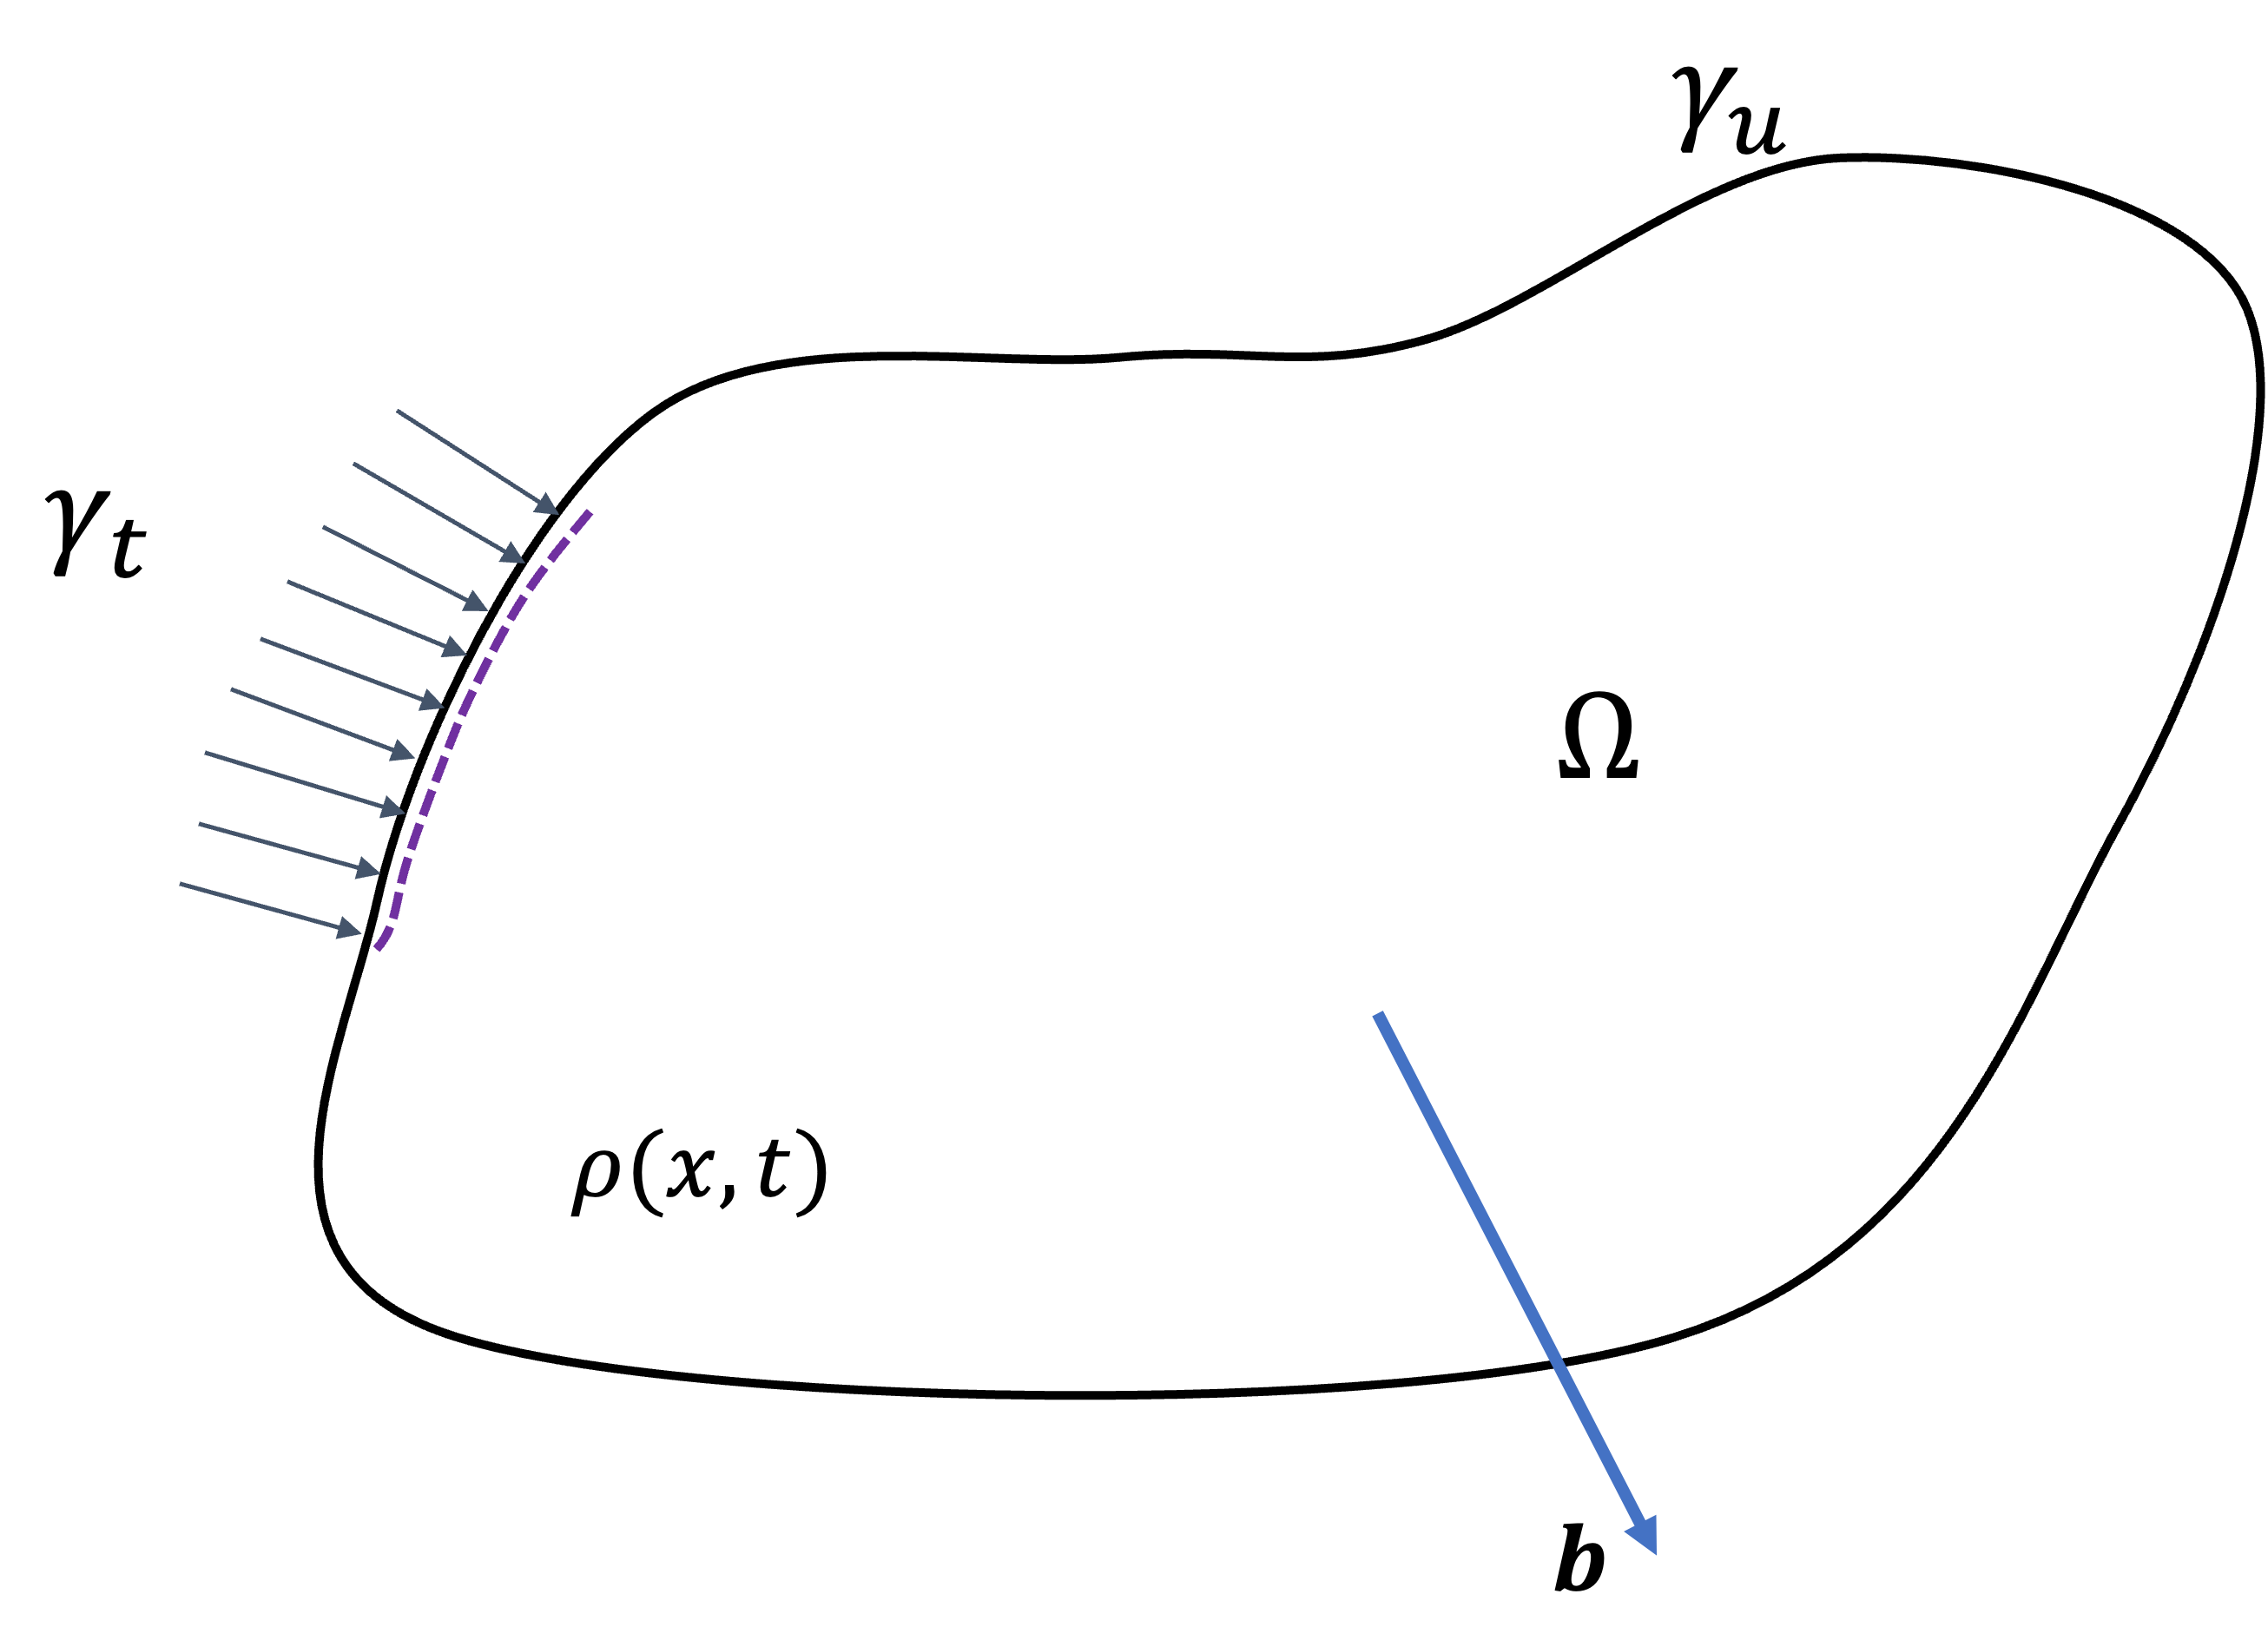
\includegraphics[width=0.4\textwidth]{./PICS/MPMEq.png}
\caption{Various stages in MPM computations}
\label{Fig:MPM_Dom}
\end{figure}
For a continuum body occupying a region $\Omega$ in space and bounded by a surface $\Gamma=\Gamma_u \cup \Gamma_t$ as shown in Figure~\ref{Fig:MPM_Dom}, the total mass $m$ of the body is given by,
\begin{align}
m=\int_{\Omega} \rho(\mathbf{x}, t) d V
\end{align}
where $\rho$ is the density of the material.

Since the mass contained in the region $\Omega$ and moving with local velocity is constant, the total time derivative is zero. Hence,
\begin{align}
\frac{\mathrm{D}}{\mathrm{D} t} \int_{\Omega} \rho(\mathbf{x}, t) \mathrm{d} V=\int_{\Omega}(\dot{\rho}+\rho \nabla \cdot \boldsymbol{v}) \mathrm{d} V=0
\end{align}

which leads to the mass conservation equation as,
\begin{align}
\rho J-\rho_0=0
\end{align}

\subsection{Conservation of momentum}
The Newton's second law of motion states that the rate of change of momentum of a body is equal to the sum of volume and surface forces acting on it. Consider the same body as shown in Figure~\ref{Fig:MPM_Dom}, with a body force per unit mass $\mathbf{b}$ and traction $\mathbf{t}$ acting on it's surface. The law of conservation of momentum is expressed as,
\begin{align}
\frac{\mathrm{D}}{\mathrm{D} t} \int_{\Omega} \rho \mathbf{v} \mathrm{d} V=\int_{\Omega} \rho \mathbf{b}(\mathbf{x},t) \mathrm{d} V + \int_{\Gamma_t} \mathbf{t}(\mathbf{x},t).\mathbf{n} \mathrm{d} A
\end{align}

By invoking the Reynolds transport theorum and upon simplifying one obtains,
\begin{align}
\rho \dot{\mathbf{v}} = \rho \mathbf{b} + \nabla . \sigma 
\end{align}


\subsection{Initial and Boundary conditions}
Two types of boundary conditions are considered in MPM solution, namely boundaries with specified velocity and specified traction respectively.
\begin{align}
& \left\{\begin{array}{l}
\left.(\boldsymbol{n} \cdot \boldsymbol{\sigma})\right|_{\Gamma_t}=\overline{\boldsymbol{t}} \\
\left.\boldsymbol{v}\right|_{\Gamma_u}=\overline{\boldsymbol{v}}
\end{array}\right. \\
\end{align}
Initial conditions in MPM involve specifying displacement of material points and velocities at time t=0.
\begin{align}
& \mathbf{v}(\mathbf{x}, 0)=\mathbf{v}_0(\mathbf{x}), \quad \mathbf{u}(\mathbf{x}, 0)=\mathbf{u}_0(\mathbf{x})
\end{align}

